\documentclass{beamer}
\usetheme{Montpellier}
\usecolortheme{dolphin}

%\usepackage{graphicx} %For jpg figure inclusion
%\usepackage{times} %For typeface
%\usepackage{epsfig}
\usepackage{color} %For Comments
\usepackage{beamerthemeshadow} %Paul and Lemmon put this in, take out if you want
%\usepackage[all]{xy}
%\usepackage{float}
%\usepackage{subfigure} 
%\usepackage{hyperref}
%\usepackage{url}
%\usepackage{parskip}
%\usepackage{multirow}

%% Elena's favorite green (thanks, Fernando!)
\definecolor{ForestGreen}{RGB}{34,139,34}
\definecolor{BlueViolet}{RGB}{138,43,226}
\definecolor{Coquelicot}{RGB}{255, 56, 0}
\definecolor{Teal}{RGB}{2,132,130}
\definecolor{PrettyGreen}{RGB}{48,197,48}
% Uncomment this if you want to show work-in-progress comments
\newcommand{\comment}[1]{{\bf \tt  {#1}}}
% Uncomment this if you don't want to show comments
%\newcommand{\comment}[1]{}
\newcommand{\emcomment}[1]{\textcolor{ForestGreen}{\comment{Elena: {#1}}}}
\newcommand{\todo}[1]{\textcolor{blue}{\comment{To Do: {#1}}}}
\newcommand{\pscomment}[1]{\textcolor{Coquelicot}{\comment{Paul: {#1}}}}
\newcommand{\mmcomment}[1]{\textcolor{magenta}{\comment{Max: {#1}}}}
\newcommand{\escomment}[1]{\textcolor{BlueViolet}{\comment{Emma: {#1}}}}
\newcommand{\alcomment}[1]{\textcolor{red}{\comment{Lemmon: {#1}}}}
\newcommand{\hfcomment}[1]{\textcolor{Teal}{\comment{Henry: {#1}}}}
%%%%%%%%%%%%%%%%%%%%%%%%%%%%%%%%%%%%%%%%%%

\begin{document}
\title{Developing Beginner-Friendly User Interactions for the Clojure Programming Language}
\date{April 11, 2015}

\begin{frame}
\frametitle{Developing Beginner-Friendly User Interactions for the Clojure Programming Language}
{\centering
\noindent
Henry Fellows, Aaron Lemmon, Max Magnuson, \par
Emma Sax, Paul Schliep, and Elena Machkasova \par

{\it 
Midwest Instruction and Computing Symposium\par
April 11, 2015\par}
}
\end{frame}
%frame

\begin{frame}
\frametitle{Table of contents}
\tableofcontents  
\end{frame}

\section{Introduction to the Project}
\begin{frame}
	\frametitle{Clojure in an introductory course}
	\begin{itemize}
		\item Developed in 2007 by Rich Hickey
		\item In the Lisp family
		\item Felleisen et al found Lisp languages to be useful in introductory courses
	\end{itemize}
\end{frame}

\begin{frame}
\frametitle{Motivations for the project}
	\begin{itemize}
		\item ClojurEd
			\begin{itemize}
				\item ongoing project
				\item introduce Clojure in an introductory course
			\end{itemize}
		\item Our work focuses on error messages in Clojure
			\begin{itemize}
				\item focus on usability
				\item error messages useful learning tool
			\end{itemize}
	\end{itemize}
\end{frame}

\section{Overview of Clojure}

\begin{frame}
\frametitle{Overview of Clojure}
	\begin{itemize}
  	 \item Dynamically typed
  	 \item Functional
  	 \item Runs on the Java Virtual Machine (JVM)
  	 \item Read-eval-print-loop (REPL)
  	 \item Data types immutable by default
	 \end{itemize}
\end{frame}

\begin{frame}[fragile]
\frametitle{Prefix notation}
	\begin{itemize}
  	  \item Clojure uses prefix notation
  	  \begin{itemize}
  	 	 \item parentheses
  	 	 \item parameters
  	  \end{itemize}
		 
	  \texttt{(<function-name> <argument 1> <argument 2>)}
	  
	  \begin{itemize}
  	 	\item a simple example
  	 	\begin{itemize}
  	 	   \item \texttt{+} is a built-in function, not an operation
  	 	\end{itemize}
  	 	\begin{verbatim}		
		(+ 5 5)
		-> 10
	        \end{verbatim}
  	  \end{itemize}
   \end{itemize}
\end{frame}

\begin{frame}[fragile]
\frametitle{Defining functions and variables}
	\begin{itemize}
  	  \item \texttt{def} can be used to define variables:
  	  \begin{verbatim}
		 (def my-string "Hello World")
		 my-string
		 -> "Hello World"
	  \end{verbatim}
  	  \item \texttt{defn} can be used to define functions:
  	  \begin{verbatim}
		 (defn increment-number [number] (+ number 1))
		 (increment-number 2)
		 -> 3
	  \end{verbatim}
	\end{itemize}
\end{frame}

\begin{frame}[fragile]
\frametitle{Collections}
    \begin{itemize}
         \item All collections can contain any number of values of any data type
         
	 \begin{itemize}
	   \item lists
	   
	   \begin{verbatim}(1 2 "foo" :a 9 "bar")
	   \end{verbatim}
	   
  	   \item vectors
  	   
  	   \begin{verbatim}[1 2 "foo" :a 9 "bar"]
	   \end{verbatim}
  	   \item hashmaps (key-value pairs)
  	   
  	   \begin{verbatim}{:a 1, :b 2, :c 3}
	   \end{verbatim}
	 \end{itemize}
    \end{itemize}
\end{frame}

\begin{frame}[fragile]
\frametitle{Anonymous functions}
	\begin{itemize}
  	  \item Anonymous functions are a way to implement a function on the fly, and use it only once
  	  \begin{itemize}
  	    \item a simple example
  	    \begin{itemize}
  	 	  \item \texttt{map} takes a function and a collection as arguments, and applies the function to the entire collection
  	    \end{itemize}
  	    
		\texttt{(map (fn [number] (+ number 1)) [0 1 2 3])}
		
		\texttt{-> (1 2 3 4)}
	 \end{itemize}
   \end{itemize}
\end{frame}

\begin{frame}[fragile]
\frametitle{Lazy sequences}
	\begin{itemize}
  	  \item Only a needed portion of a sequence is evaluated
	  \begin{itemize}
  	     \item a simple example
  	     \begin{itemize}
  	         \item \texttt{take} takes the first $n$ elements of a collection
  	         \item \texttt{range} returns an infinite sequence of non-negative integers beginning at 0
  	     \end{itemize}
  	     \texttt{(take 10 (range))}
  	 	      
  	     \texttt{-> (0 1 2 3 4 5 6 7 8 9)}
  	     \item Fibonacci sequence
  	   \end{itemize}
   \end{itemize}
\end{frame}

\section{Error Messages}

\begin{frame}
\frametitle{Clojure error messages: background}
	\begin{itemize}
  		\item Error messages should be:
  		\begin{itemize}
  	 		\item helpful for debugging
  	 		\item easy to understand
  	 		\item not intimidating
  		\end{itemize}
  		\item Clojure error messages are confusing
	 \end{itemize}
	 
\end{frame}

\begin{frame}[fragile]
\frametitle{Clojure error messages: examples}

\begin{itemize}
	\item \begin{verbatim}
EOF while reading, starting at line 3, 
compiling:(compilation_errors/eof.clj:4:1)
\end{verbatim}

	\item \begin{verbatim}
IllegalArgumentException Parameter declaration
	* should be a vector 
	clojure.core/assert-valid-fdecl (core.clj:6842)
\end{verbatim}

\item \begin{verbatim}
ClassCastException java.lang.String cannot be
cast to clojure.lang.IPersistentCollection 
clojure.core/conj (core.clj:83)
\end{verbatim}

\end{itemize}

\end{frame}

\begin{frame}
\frametitle{Error message transformation: approaches}
	\begin{itemize}
	 	\item Function substitution approach
	 		\begin{itemize}
  	 			\item add type-checking preconditions
  	 			\item type mismatch produces custom message
	 		\end{itemize}
	 
		\item Try/catch approach
			\begin{itemize}
  				\item wrap user's code in try/catch block
  				\item capture error message
  				\item check against collection of regular expressions
  				\item replace with improved message
			\end{itemize}
	\end{itemize}
\end{frame}

\begin{frame}[fragile]
\frametitle{Error message transformation: discussion}

	\begin{itemize}
		\item Function substitution approach
			\begin{itemize}
				\item able to recover argument values and use them for a more meaningful message
				\begin{verbatim}
				(+ 2 "apple")
				\end{verbatim}
				\textcolor{PrettyGreen}{
				\texttt{
				-> ERROR: In function +, the second argument
				"apple" must be a number but is a string.
				}}
				\item unable to handle compilation exceptions
				\item can not handle user-made functions
				\item impractical to redefine all existing functions
			\end{itemize}
		\item Try/catch approach
			\begin{itemize}
	 			\item able to handle both runtime and compilation exceptions
				\item usually can not recover argument values
	 		\end{itemize} 
	\end{itemize}
\end{frame}

\begin{frame}[fragile]
\frametitle{User scenarios: example slide 1}

	\begin{itemize}
		\item Erroneous code fragment:
			\begin{verbatim}
			print(Hello World)
			\end{verbatim}
			
		\item Clojure error message:
			\begin{verbatim}
			CompilerException java.lang.RuntimeException:
			Unable to resolve symbol: Hello in this context
			\end{verbatim}
			
		\item Our improved error message:
		
			\textcolor{PrettyGreen}{
			\texttt{ERROR: Compilation error: name Hello is undefined}
			}
		\item Student edit
		
				\texttt{print(\alert{"Hello World"})}
	\end{itemize}
	
\end{frame}

\begin{frame}[fragile]
\frametitle{User scenarios: example slide 2}

	\begin{itemize}
	\item Student edit
		
				\texttt{print("Hello World")}
				
		\item Clojure error message:	
	
			\begin{verbatim}
			ClassCastException java.lang.String cannot be
			cast to clojure.lang.IFn
			\end{verbatim} 
	
		\item Our improved error message:	
	
			\textcolor{PrettyGreen}{
			\texttt{ERROR: Attempted to use a string, but a function
			was expected.}}
	
		\item Corrected Code:
		
			\texttt{\alert{(print} "Hello World")}
	\end{itemize} 	

\end{frame}

\begin{frame}
\frametitle{User scenarios: explanation}
	\begin{itemize}
  	 \item Explore common use cases
  	 \item Discover which errors occur
  	 \item Develop useful hints
	 \end{itemize}
\end{frame}

\begin{frame}
\frametitle{Hints: how they are helpful}
	\begin{itemize}
  	 \item Errors can have several underlying causes
  	 \item Multiple hints per error
  	 \item Provide more human interpretation of the issue
  	 \item Offer suggestions on how to resolve issues
	 \end{itemize}
\end{frame}

\begin{frame}[fragile]
\frametitle{Hints: example}

	\begin{itemize}
		\item Erroneous code fragment:
		
			\texttt{print(Hello World)}

		\item Clojure error message:
		
  			 \begin{verbatim}
	CompilerException java.lang.RuntimeException:
Unable to resolve symbol: Hello in this context
			\end{verbatim}
			
		\item Improved error message
		
			\textcolor{PrettyGreen}{
			\texttt{ERROR: Compilation error: name Hello is undefined}}
			
		\item Hint:
		
			\begin{verbatim}
	It looks like Clojure is expecting that Hello is
	something named in your program. If you wanted Hello
	and any following words to be plain text, try
	surrounding them with double quotes. If Hello is
	referring to something named in your program, make
	sure it is spelled correctly.
			\end{verbatim}
	
	\end{itemize}
\end{frame}

\begin{frame}
\frametitle{Hints: future work}
	\begin{itemize}
  	 \item Develop more user scenarios
  	 \item Usability study with students
  	 \item Provide links to Clojure documentation
	 \end{itemize}
\end{frame}

% Henry & Max
\section{Technical Setup}

\begin{frame}
\frametitle{Setup}
	\begin{itemize}
		\item IDE options
		\begin{itemize}
			\item LightTable
			\item Nightcode
		\end{itemize}
		\item Project manager
		\begin{itemize}
			\item Leiningen
			\item popular in Clojure community
		\end{itemize}
	\end{itemize}
\end{frame}

\begin{frame}
	\frametitle {Differences in error handling}
	\begin{itemize}
		\item Runtime, compile time, REPL
		\item Consistency
		\item Laziness
		\item Try/catch does not catch all
	\end{itemize}
\end{frame}

\begin{frame}[fragile]
\frametitle{Current workflow diagram}
\begin{figure}[h]
 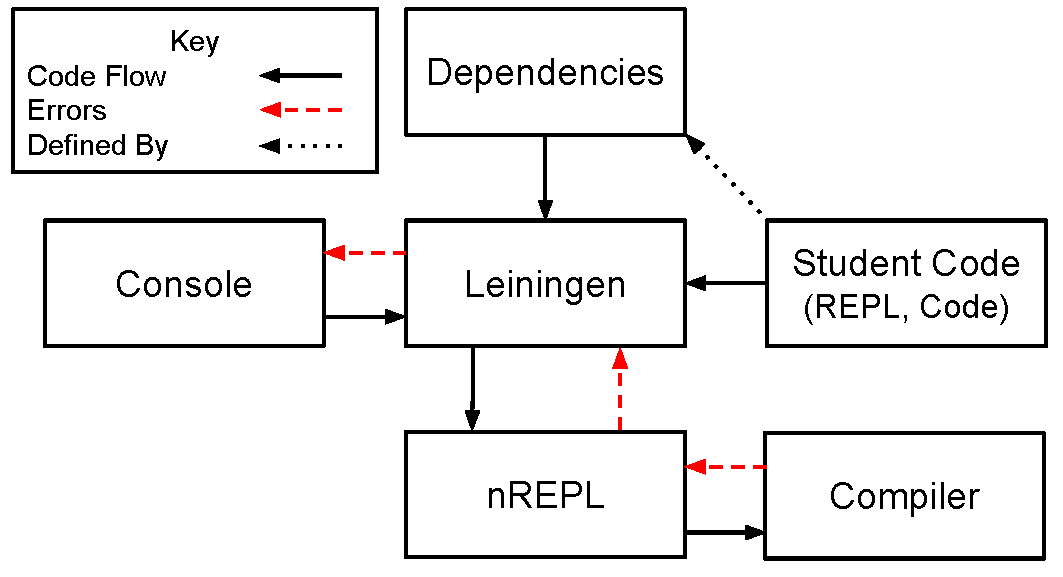
\includegraphics[width=10cm]{../CurrentErrorHandling.pdf}
 \centering
\end{figure}
\end{frame}

\begin{frame}
\frametitle{Issues}
	\begin{itemize}
		\item Installation of Leiningen is nontrivial
		\item Command line acts as a barrier
		\item We do not want students managing dependencies
		\item No integration with new error handling system
	\end{itemize} 
\end{frame}

\begin{frame}
\frametitle{Future work}
	\begin{itemize}
		\item Use scripting to abstract over Leiningen installation
		\item Graphical User Interface will abstract over command line
		\item Leiningen plugin to inject needed dependencies
		\item Use nREPL to integrate new error handling system
	\end{itemize}
\end{frame}

\begin{frame}[fragile]
\frametitle{Proposed workflow diagram}
\begin{figure}[h]
 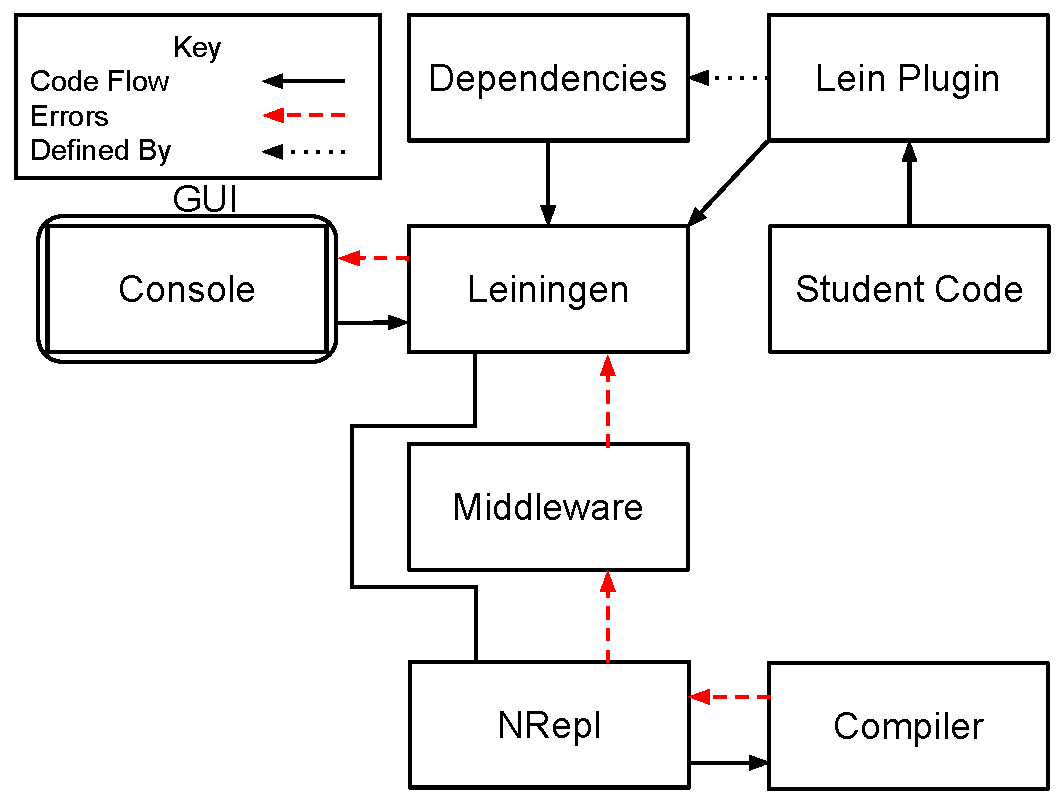
\includegraphics[width=9cm]{../OurErrorHandlingSystem.pdf}
 \centering
\end{figure}
\end{frame}

\begin{frame}
\frametitle{What needs to be done}
\begin{itemize}
	\item These solutions are a work in progress
	\item The system still needs implementation
	\item The proposed solution is a result of our findings
\end{itemize}
\end{frame}

\end{document}

